\documentclass[a4paper,12pt]{article} 
\usepackage[top = 2.5cm, bottom = 2.5cm, left = 2.5cm, right = 2.5cm]{geometry} 
\usepackage[T1]{fontenc}
\usepackage{multirow} 
\usepackage{amsmath}
\usepackage{booktabs} 
\usepackage{graphicx} 
\usepackage{setspace}
\usepackage{float}
\usepackage{fancyhdr}
\usepackage{fancybox}
\usepackage{graphicx}
\usepackage[framemethod=tikz]{mdframed}
\usetikzlibrary{shadows}

\newmdenv[shadow=true,shadowcolor=black,font=\sffamily,rightmargin=8pt]{shadedbox}


\pagestyle{fancy}

\fancyhf{}

\lhead{\footnotesize Inv. de Operaciones: Tarea Final}

\rhead{\footnotesize Martin Mancilla, Claudio Duran}

\cfoot{\footnotesize \thepage} 

\begin{document}
	
\thispagestyle{empty}

\begin{tabular}{p{15.5cm}}
	{\large \bf Investigación de Operaciones} \\
	Universidad Católica del Maule \\ Martín Mancilla V. - Claudio Durán N.\\
	\textit{19.386.399-k} - \textit{19.215.697-1} \\
	\hline
	\\
\end{tabular}

\vspace*{0.3cm}

\begin{center}
	{\Large \bf Trabajo Final} 
	\vspace{2mm}
	
	% YOUR NAMES GO HERE
	{Resolución de Problemas de Optimización}
	
\end{center}  

\vspace{0.4cm}

\section{Primer Problema}
\subsection{Formule  el  modelo  que  permita  obtener  el  portafolio de  inversión  que  optimice  el  retorno  esperado  de  la	corporación y simultáneamente no viole su política de inversión}
\subsubsection{Variable de Decisión}
\begin{equation*}
	\begin{split}
		N &= \{1,2,3,4,5\} \\
		X_i & = \text{Cantidad invertida en categoría } i \text{ de la inversión. } \forall i \in N
	\end{split}
\end{equation*}
\begin{center}
	\noindent\rule{12cm}{0.4pt}
\end{center}
\begin{shadedbox}
1 = Acciones comunes, 2 = Cuotas de fondos mutuos, 3 = Bonos de Oferta Pública,\\ 4 = Bonos de Gobierno, 5 = Cuentas de Ahorro
\end{shadedbox}
\subsubsection{Constantes}
\begin{equation*}
\begin{split}
	RAE &= [0.15,\ 0.12,\ 0.10,\ 0.05,\ 0.08] \\
	FR & = [1.6,\ 1.0,\ 0.5,\ 0.0,\ 0.1] \\
	RAE_i &= \text{ Retorno Anual Esperado para la categoría } i \text{ de la inversión } \forall i \in N. \\
	FR_i &= \text{Factor de riesgo para la categoría } i \text{ de la inversión } \forall i \in N.
\end{split}
\end{equation*}
\subsubsection{Función Objetivo}
\begin{equation*}
\begin{split}
	maxZ = \sum_{i = 1}^{i}X_i\times RAE_i
\end{split}
\end{equation*}
\subsubsection{Restricciones}
\begin{enumerate}
	\item La inversión en acciones y en cuotas de fondos mutuos no debe ser mayor que un
	30\% del total de  las  inversiones.
	\begin{equation*}
		x_1 + x_2 \leq 0.3\times\sum_{i = 1}^{i}x_i
	\end{equation*}
	\item La  inversión  en  bonos  de  gobierno  no  debe  ser  inferior  a  la  inversión  en  cuentas  de  ahorro.
	\begin{equation*}
		x_4 \geq x_5
	\end{equation*}
	\item La inversión en debentures y bonos de gobierno no debe exceder el 50\% del total de las inversiones.
	\begin{equation*}
		x_3 + x_4 \leq 0.5\times\sum_{i = 1}^{i}x_i
	\end{equation*}
	\item La inversión en bonos de gobierno debe superar el 25\% del total de las inversiones.
	\begin{equation*}
		x_4 \geq 0.25\times\sum_{i = 1}^{i}x_i
	\end{equation*}
	\item La corporación Gamma    requiere invertir  la  suma  de  US\$  1.000.000  en el  próximo  año  fiscal.
	\begin{equation*}
		\sum_{i = 1}^{i}x_i \leq 1,000,000
	\end{equation*} 
	\item La corporación  no  permite  que el  portafolio  de  valores  escogidos  tenga  un  factor de  riesgo ponderado mayor que 1.0.
	\begin{equation*}
		\sum_{i = 1}^{i}x_i\times FR_i \leq \sum_{i = 1}^{i}x_i
	\end{equation*}
	\item No negatividad.
	\begin{equation*}
		x_i\geq 0\ \forall i \in N
	\end{equation*}
\end{enumerate}
\newpage
\section{Segundo Problema}
\subsection{Dibuje el grafo que represente el problema.}
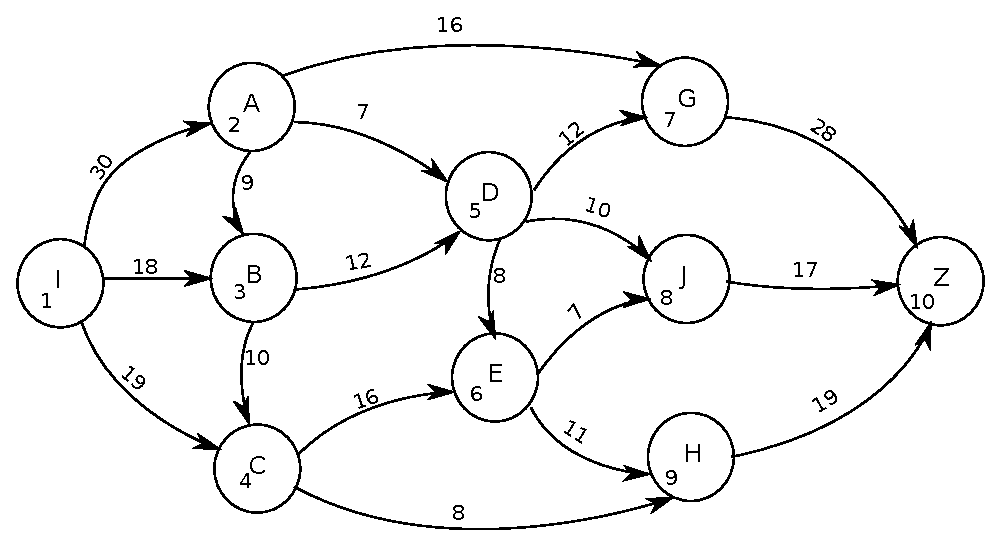
\includegraphics[scale=1]{drawing.eps}
\subsection{Formule el modelo que le permite resolver este problema}
\subsubsection{Nodos y Aristas}
\begin{equation*}
\begin{split}
	N = &\{1,2,3,4,5,6,7,8,9,10\} \\
	A = &\{ (1,2)(1,3)(1,4)(2,3)(2,5)(2,7)(3,4)(3,5)(4,6)\\
	  &(4,9)(5,6)(5,8)(6,8)(6,9)(7,10)(8,10)(9,10) \}
\end{split}
\end{equation*}
\subsubsection{Variable de Decisión}
\begin{equation*}
\begin{split}
	X_{ij} &= \text{Cantidad de mensajes transmitidos de nodo } i \text{ a nodo } j \ (\forall(i,j)\in A)\\
	v &= \text{Flujo máximo de los nodos}
\end{split}
\end{equation*}

\subsubsection{Función Objetivo}
\begin{equation*}
	maxZ = v
\end{equation*}

\subsubsection{Restricciones}
\begin{itemize}
	\item Oferta
		\begin{equation*}
		\text{(1) }	X_{12}+X_{13}+X_{14}=v	
		\end{equation*}
	\item Demanda
		\begin{equation*}
		\text{(10)}	-X_{71}-X_{810}-X{910}=-v
		\end{equation*}
	\item Transición
		\begin{equation*}
		\begin{split}
			(2)&X_{23}+X_{25}+X_{27}-X_{12}=0\\
			(3)&X_{34}+X_{35}-X_{13}-X_{23}=0\\
			(4)&X_{46}+X_{49}-X_{14}-X_{34}=0\\
			(5)&X_{56}+X_{57}+X_{58}-X_{25}-X_{35}=0\\
			(6)&X_{68}+X_{69}-X_{46}-X_{56}=0\\
			(7)&X_{710}-X_{27}-X_{57}=0\\
			(8)&X_{810}-X_{58}-X_{68}=0\\
			(9)&X_{910}-X_{49}-X_{69}=0
		\end{split}
		\end{equation*}
		\item Capacidad de aristas
		\begin{equation*}
		\begin{split}
			X_{12}&\leq 30 \qquad X_{34}\leq 10 \qquad X_{58}\leq 10\\
			X_{13}&\leq 18 \qquad X_{35}\leq 12 \qquad X_{68}\leq 7\\
			X_{14}&\leq 19 \qquad X_{46}\leq 16 \qquad X_{69}\leq 11\\
			X_{23}&\leq 9 \qquad X_{49}\leq 8 \qquad X_{710}\leq 28\\
			X_{25}&\leq 7 \qquad X_{56}\leq 8 \qquad X_{810}\leq 17\\
			X_{27}&\leq 16 \qquad X_{57}\leq 12 \qquad X_{910}\leq 19\\
		\end{split}
		\end{equation*}
		\begin{equation*}
			X_{ij}\geq 0\ \forall(i,j)\in A
		\end{equation*}
\end{itemize}
\end{document}